\chapter{Epidemic Modelling}
\label{ch:progress}

\section{Motivations}
Modelling, is a technique commonly used in order to approximate an environment/system to gain insights and better understand possible outcome scenarios especially in situations when we don't have data available about the topic. Some examples of applications in which modelling is commonly applied are: climate change, military defense, designing cities, infecting diseases development and testing financial policies. 

Using modelling simulations, can be of great help when trying to answer different types of causal questions about our research topic (e.g. varying the different simulation parameters, it can be possible to see how these are related each other and how they affect the overall outcome). 

As part of this study, an interactive online Web Application \footnote{Web Application Link: \url{http://3.22.240.181:8501/}} has been developed in order to quickly analyse in real time COVID-19 developments and simulating different scenarios and approaches which can be taken in order to mitigate the consequences of this outbreak. Most of the provided models have been designed so that to be flexible enough to model any other type of possible future infectious disease. 

Additionally, a secondary website has been created using GitHub Pages in order to share additional notebooks and animations in Python and Julia \footnote{GitHub Pages Website Link: \url{https://pierpaolo28.github.io/Epidemics-Modelling/}}. 

\section{Introduction to Epidemiology}

\subsection{Different Classes of Diseases}
Infectious diseases, can mainly be classified into three different categories depending on their characteristics \cite{2minclass}:
\begin{enumerate}
    \item \textbf{Endemic}: an endemic is an health concern which is constantly present at a low rate within a population (its presence doesn't either substantially increase or decline). Some examples of endemics are Malaria and Chicken Pox.
    \item \textbf{Epidemic}: is an health issue which can cause a fast and unforeseen increase in cases within a population. An example of epidemic, can be considered the seasonal flu, which can lead to a sharp increase in the number of infected at specific times of the year.
    \item \textbf{Pandemic}: epidemics can finally later become pandemics if they manage to spread around the world and effect a great number of people. Some examples of pandemics are the Spanish Flu and COVID-19.
\end{enumerate}

\subsection{Exponential vs Logistic Growth}
\label{explog}
Pandemics, usually develops thanks to a disease ability to spread at an exponential rate. In the case of COVID-19, the number of cases from one day to the next was in fact equal to the number of nowadays cases times some constant between 1.25-1.5 (depending on factors such as population density and restrictions in place). The change in the number of cases from a day to another, can then be defined by the following equation \cite{exponentials}:

\useshortskip
\begin{align}
\ \Delta N_{d} = E \times p \times N_{d}
\label{n_new}
\end{align}
\useshortskip

Where $E$ represents the average number of people we are exposed to every day, $p$ represents the probability that an exposure might lead to an infection and $N_{d}$ is the number of cases as of today. Therefore, in this type of situation, the only possible way to try to slow down our exponential trend is by decreasing $E$ and $p$. In order to make this possible, different techniques such as track and trace, social distancing and travel restrictions can be applied. Although, even if no intervention at all is done, an exponential trend is destined to convert to a logistic curve once a large number of the population gets infected by the disease (in fact, the probability than an exposure can lead to an infect automatically decreases if the majority of the population and the people we meet are already infected). Applying any type of restriction, would then help us in making possible to reach our inflection point between these two trends as soon as possible.

Exponential growths, can be easier to inspect if when plotting them on a logarithmic scale. Using this type of graph, an exponential curve would then look like approximately a straight line. As we can see from the graph on the left of Figure \ref{exp}, all the different considered countries follow the at first the same exponential pattern which then seems to be starting converting to a logistic curve. The graph on the right of Figure \ref{exp}, was then designed in order to try to amplify this change \cite{physics}. While going through an exponential growth, it can be difficult to understand how long will it last (if the growth is going to still keep being exponential or is going to start decaying). One possible way to approach this problem, is to focus our attention on the rate of change in new cases from a week to another. Plotting this on a both axis logarithmic scale, we would then clearly see that all the different countries have a same linear growth in cases. Although, using some form of containment, some of these countries are successfully able to escape from this linear growth in cases. Using this type of approach, we can successfully emphasize the deviation in the growth of an exponential curve.

\begin{figure}[ht!]%
    \centering
    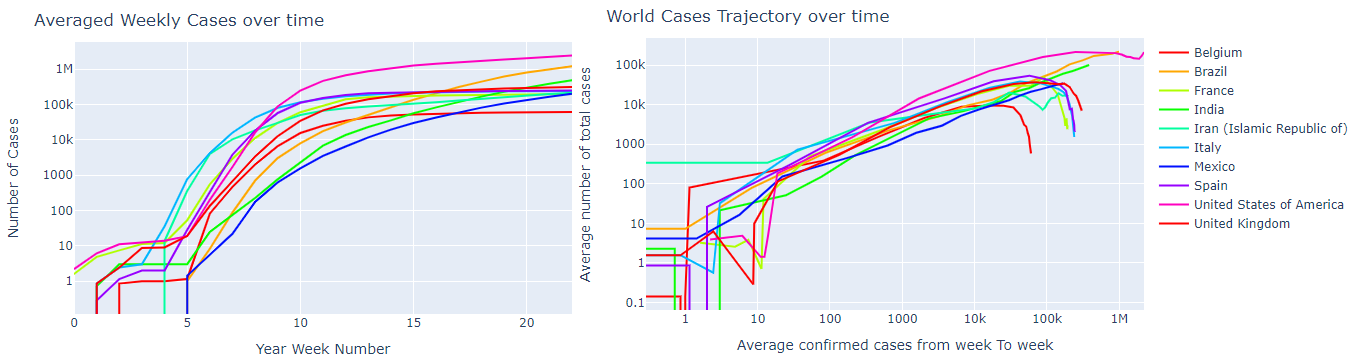
\includegraphics[width=17cm]{latex/images/logplot.png}%
    \caption{Exponential Growth Evolution}
    \label{exp}
\end{figure}

Using the logarithmic linear graphs, we could then perform a linear regression to find the line of best fit and find out how many days does it take for our cases to increase by a fixed constant. Finally, using metrics such as the $R^{2}$ score, we could then quantitatively measure how far are our curves from an exponential curve.

Another way to examine if we are reaching the end of an exponential curve, is by examining the slope (Growth Factor, Equation \ref{growth}).

\useshortskip
\begin{align}
\ Growth \; Factor = \dfrac{\Delta N_{d}}{\Delta N_{d-1}}
\label{growth}
\end{align}
\useshortskip

A growth factor of more than one, will show us that we are still going through an exponential growth, while a growth factor equal to 1 can tell us we might now be approaching our inflection point.

\subsection{Quantifying the spread of a disease}
One of the main unit used to measure how easily a disease is able to diffuse in a community is the "Effective Reproductive Number" ($R$), which is measured as the average number of people infected by each individual carrying the disease. In a fully susceptible population, $R$ is also referred as $R_{0}$ ("Basic reproductive Number"). The Basic reproductive Number for COVID-19 is currently estimated to be around 2.5.

As shown in Equation \ref{r0}, $R_{0}$ can be calculated as the number of people someone positive to the disease can infect each day ($\beta$) multiplied by the number of days each person remains positive to the disease ($D$). Equivalently, $R_{0}$ can also be estimated as the number of people someone positive to the disease can infect each day multiplied by the proportion of individuals infected recovering each day ($\gamma = 1/D$). Furthermore, as shown in Equation \ref{day_inf}, $\beta$ can be also calculated to be equal to the probability that an exposure might lead to an infection ($p$) multiplied by the average number of people we are exposed to every day ($E$) \cite{tds}.

\useshortskip
\begin{align}
\ R_{0} = \beta \times D = \beta \times \gamma
\label{r0}
\end{align}
\useshortskip

\useshortskip
\begin{align}
\ \beta = E \times p
\label{day_inf}
\end{align}
\useshortskip

If $R$ is greater than one, then the disease is still in the exponentially growing phase (we have an epidemic), if $R$ is instead equal to one we are instead in an endemic (therefore the number of cases stays approximately constant) and if $R$ is less than one, we are instead in the eradication phase and the disease could disappear entirely soon from our population.

One of the most common approaches to eradicate a decease, is through Herd Immunity. The percentage proportion of the individuals in a population necessary to reach Herd Immunity can be estimated using Equation \ref{immunity}. In the case of COVID-19, this is estimated to be around 60\%. Herd Immunity, can potentially be achieved either through vaccination or natural selection \cite{blob}.

\useshortskip
\begin{align}
\ Herd\:Immunity\:(H.I.) = 1 - \frac{1}{R_{0}}
\label{immunity}
\end{align}
\useshortskip

Different typology's of Epidemics Modelling have been developed in the past few years, such as:
\begin{itemize}
    \setlength\itemsep{-0.3cm}
    \item Compartmental Models
    \item Agent Based Models
    \item Network Models
    \item Meta-populations Models
\end{itemize}

In this chapter, we will explore the first two approaches.

\section{Compartmental Models}

In Compartmental Models, is assumed that each individual in a population, is assigned to a compartment. During the course of the simulations, individuals can then be free to move from one compartment to another depending on the dynamics of the model. Some examples of common departments in Epidemic Modelling are: Susceptible, Exposed, Infectious, Recovered, Dead, Vaccinated, etc...

This models can be designed using either ordinary differential equations or stochastic elements as well. Diagrams representations of this type of models can be of great help in order to understand how the model equations works and what are the possible movements between different states. 

\subsection{SIR (Susceptible-Infected-Recovered)}

The SIR model can be described by the following three formulas, where 
$N$ is the total number of elements in the population, $\beta$ represents average amount of people an infected element can be able to infect in a day and
$\gamma$ the percentage of how many individuals recover from the disease each day.

\useshortskip
\begin{align}
\ \frac{\partial S}{\partial t} = -\beta \times I \times \frac{S}{N}
\end{align}
\useshortskip

\useshortskip
\begin{align}
\ \frac{\partial I}{\partial t} = \beta \times I \times \frac{S}{N} -\gamma \times I
\end{align}
\useshortskip

\useshortskip
\begin{align}
\ \frac{\partial R}{\partial t} = \gamma \times I
\end{align}
\useshortskip

Using the parameters in Table \ref{table:1}, it can then be possible to obtain the results in Figure \ref{sir}.

{
\begin{table}[h!]
\centering
\begin{tabular}{|c|c|}
\hline
Parameter Type & Value \\
\hline
Population Size & 100  \\
Number of Days & 100  \\
Number of individuals originally infected & 3  \\
Number of individuals at close contact in a day & 5 \\
Probability of infection if in contact with an infected & 0.1\% \\
Number of days a the disease can last & 7 \\
\hline
\end{tabular}
\caption{SIR Model Parameters}
\label{table:1}
\end{table}
}


\begin{figure}[ht!]%
    \centering
    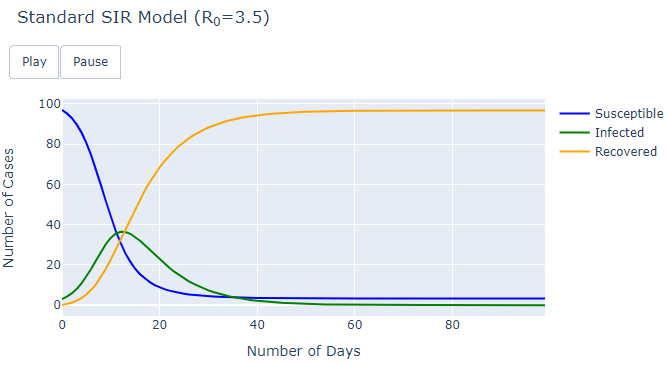
\includegraphics[width=13cm]{latex/images/sir.PNG}%
    \caption{SIR Model}
    \label{sir}
\end{figure}

\subsection{SEIR (Susceptible-Exposed-Infected-Recovered)}

In order to make our more more realistic, we can then add an additional state E representing all the population elements which are still in the incubation stage before becoming infected. In order to apply these modifications, we just need to update $\frac{\partial I}{\partial t}$ and add this extra stage before just before it. The only variable which needs to be added compared to the SIR model is $\delta$ (the percentage of how many individuals move from the incubation period to being infected).

\useshortskip
\begin{align}
\ \frac{\partial E}{\partial t} = \beta \times I \times \frac{S}{N} -\delta \times E
\end{align}
\useshortskip

\useshortskip
\begin{align}
\ \frac{\partial I}{\partial t} = \delta \times E \times -\gamma \times I
\end{align}
\useshortskip

Using the same parameters as in Table \ref{table:1}, and using one day as the number of incubation days for the disease, can then be produced the results in Figure \ref{seir}.

\begin{figure}[ht!]%
    \centering
    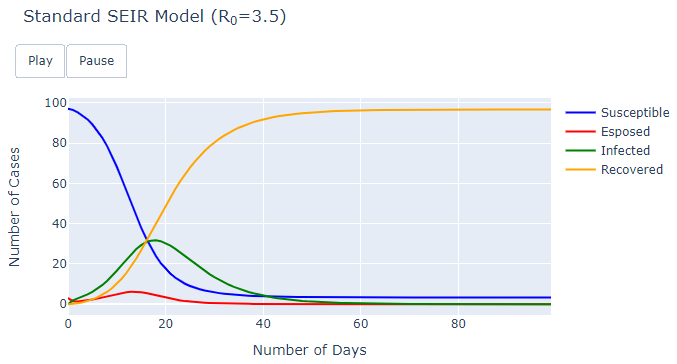
\includegraphics[width=13cm]{latex/images/seir.PNG}%
    \caption{SEIR Modelling}
    \label{seir}
\end{figure}

\subsection{Advanced SEIR Modelling}
Starting from the developed SEIR Model, it can be now possible add more compartments and make different elements time-dependent so that to better capture real-world dynamics. The main additions engineered in this model are:
\begin{itemize}
    \item Take into account the portion of infected individuals which dies instead of recover.
    \item $R_{0}$ is not anymore static but dynamically changes over time. In this example, two functions have been used  in order to simulate $R_{0}$ behaviour over time: a Sigmoid or Sinusoidal. In this way, we are now able to model
    how a government might react in order to control the spread of the disease by exercising social distancing measures. A sigmoid in it's minimum point can in fact represent a lock-down and the smoothness by which it reaches its minimum can
    easily represent how gradually the restrictions have been applied. An additional parameter is provided in order to decide from what day onward to start applying the restrictions (so that to observe what could be the consequences of a late or early intervention). The sinusoidal landscape, can instead be used in order to model possible sequential waves a disease can lead to.
    \item Also the death rate has been designed to be time and age dependent. To each different age group is assigned a different base death rate (the older, the greater), which increase linearly with the increase in the number of infected at each time-step. Therefore, with higher peaks of individuals infected all at the same time increases the likelihood of individuals to die (mimicking strained healthcare system which don't have the potential to cure everyone at the same time). An animation of how the percentage of people dying if positive ($\alpha$) varies over time, is available in the animated simulation below.
\end{itemize}

This advanced SEIR version has been inspired by Henri Froese \cite{tds} work.

\subsection{Time Limited Immunity and Vaccination Modelling}

\subsubsection{Time Limited Immunity}

Updating our SIR model, we can be able to take into account the possibility that individuals might not gain lifetime immunity from a disease when recovering from it, but that might instead be re-infected again in the future after some time. The amount of time an individual might be immune from a disease can be represented by just adding a new variable to our model ($v$).

\useshortskip
\begin{align}
\ \frac{\partial S}{\partial t} = -\beta \times I \times \frac{S}{N} + v \times R
\end{align}
\useshortskip

\useshortskip
\begin{align}
\ \frac{\partial I}{\partial t} = \beta \times I \times \frac{S}{N} -\gamma \times I
\end{align}
\useshortskip

\useshortskip
\begin{align}
\ \frac{\partial R}{\partial t} = \gamma \times I - v \times R
\end{align}
\useshortskip

Using the same SIR model parameters as in Table \ref{table:1}, setting to 25 the maximum number of days the immunity to the disease can last, we can then produce the following results in Figure \ref{low_imm}.

\begin{figure}[ht!]%
    \centering
    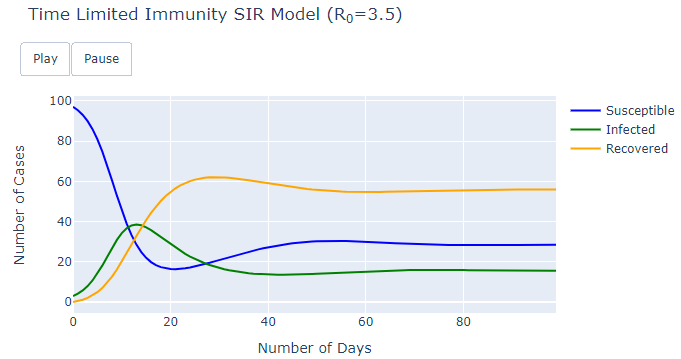
\includegraphics[width=13cm]{latex/images/time_lim.PNG}%
    \caption{Time Limited Immunity Modelling}
    \label{low_imm}
\end{figure}

\subsubsection{Vaccination}

Extending our set of equations (adding an extra stage $\frac{\partial V}{\partial t}$), we can be able to take into account how an epidemic will evolve once a vaccine is available. In order to apply these modifications, we just need to update $\frac{\partial S}{\partial t}$ and add the vaccination stage before just after it. To make the simulation more realistic, we can then also specify from when in time a vaccine could start being distributed and how fast it can produced and shipped ($p$). Finally, a stage used to record the possible amount of deaths is included (using the same notation for the SEIR and Advanced SEIR models).

\useshortskip
\begin{align}
\ \frac{\partial S}{\partial t} = -\beta \times I \times \frac{S}{N} + v \times R - p \times S
\end{align}
\useshortskip

\useshortskip
\begin{align}
\ \frac{\partial V}{\partial t} = p \times S
\end{align}
\useshortskip

\useshortskip
\begin{align}
\ \frac{\partial I}{\partial t} = -\beta \times I \times \frac{S}{N}  -(1-\alpha) \times \gamma \times I -\alpha \times \rho \times I
\end{align}
\useshortskip

\useshortskip
\begin{align}
\ \frac{\partial R}{\partial t} = (1-\alpha) \times \gamma \times I - v \times R
\end{align}
\useshortskip

\useshortskip
\begin{align}
\ \frac{\partial D}{\partial t} = \alpha \times \rho \times I
\end{align}
\useshortskip

Extending our set of parameters used for the Time Limited Immunity model, using the values from Table \ref{table:2}, has been possible to obtain the results in Figure \ref{vacc}.

{
\begin{table}[h!]
\centering
\begin{tabular}{|c|c|}
\hline
Parameter Type & Value \\
\hline
Number of days the disease can take to become lethal & 5  \\
Death rate & 0.2\%  \\
Number of Days to start Vaccine Distribution & 30  \\
Vaccine Distribution rate & 0.1\%  \\
\hline
\end{tabular}
\caption{SIR Vaccination Model Parameters}
\label{table:2}
\end{table}
}

\begin{figure}[ht!]%
    \centering
    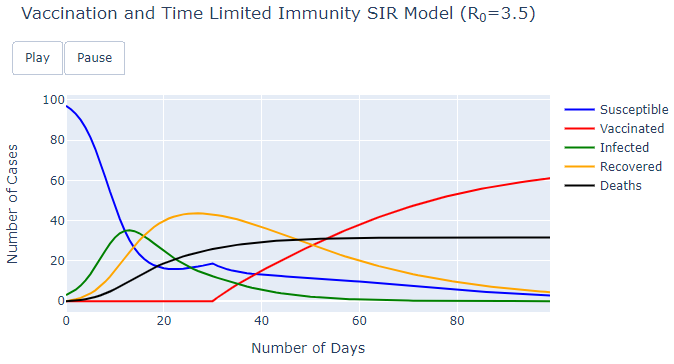
\includegraphics[width=13cm]{latex/images/vacc.PNG}%
    \caption{Vaccination Modelling}
    \label{vacc}
\end{figure}

\subsection{Coronavirus Modelling}

TODO Cite Estimated Cases paper.

\section{Agent Based Models}
An alternative approach which can be used in order to simulate compartmental-like models, is by creating an Agent Based simulation. In this case, each single individual in the population is created following an Objected Oriented Programming approach (eg. using a programming class) and it's behaviour in an environment while in contact with the rest of the population is simulated. Using this type of approach, can therefore enable us to keep track of the position of the different individuals in a population and attribute then different characteristics such as an age or daily income.

\subsection{Population Modelling}

As described in Section \ref{explog}, the number of new cases can vary according to Equation \ref{n_new}. Therefore, the only way we can be able to decrease the number of cases, is by decreasing the values of $E$ and $p$. 
\begin{itemize}
    \setlength\itemsep{-0.3cm}
    \item $E$ can decrease if travelling and meetings of people are reduced as much as possible.
    \item $p$ can be reduced instead for example by making less likely to catch the disease by taking precautions such as washing hands, wearing masks, avoid touching our faces, etc...
\end{itemize}

\begin{algorithm}
\caption{Calculate $y = x^n$}
\label{alg1}
\vspace*{-.4cm}
\begin{multicols}{2}
\begin{algorithmic}[1]
  \REQUIRE $n \geq 0 \vee x \neq 0$
  \ENSURE $y = x^n$
  \STATE $y \Leftarrow 1$
  \IF{$n < 0$}
  \STATE $X \Leftarrow 1 / x$
  \STATE $N \Leftarrow -n$
  \ELSE
  \STATE $X \Leftarrow x$
  \STATE $N \Leftarrow n$
  \ENDIF
  \WHILE{$N \neq 0$}
  \IF{$N$ is even}
  \STATE $X \Leftarrow X \times X$
  \STATE $N \Leftarrow N / 2$
  \ELSE[$N$ is odd]
  \STATE $y \Leftarrow y \times X$
  \STATE $N \Leftarrow N - 1$
  \ENDIF
  \ENDWHILE
\end{algorithmic}
\end{multicols}
\vspace*{-.3cm}
\end{algorithm}

This trend can be observed in the following proposed model by the \textbf{Contact Radius} ($E$) and \textbf{Probability of how unlikely it is to spread the virus if within the contact radius} (complementary of $p$) variables.
In this way, causal effects of social distancing and improved hygiene can be easily inspected. Furthermore, the role of dividing individuals in different communities is additionally studied. Having different communities with a central shared point and random infected initialization, can in fact resemble how contagious disease hot-spots can be created.

\begin{figure}[ht!]%
    \centering
    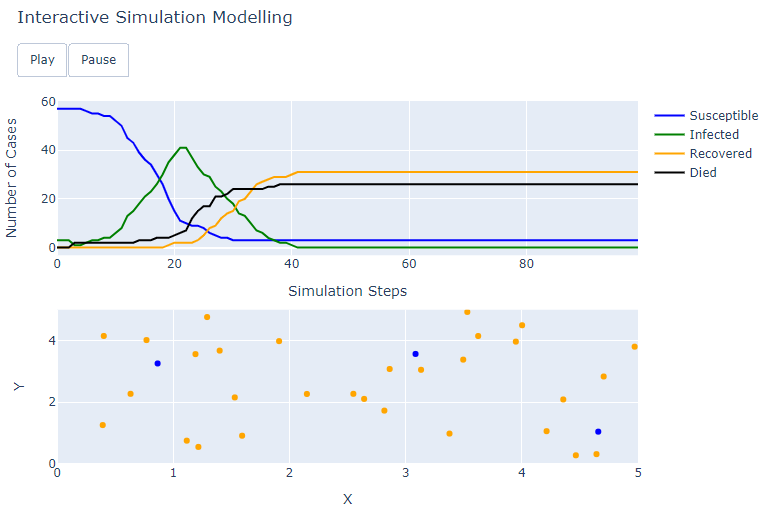
\includegraphics[width=13cm]{latex/images/pop.PNG}%
    \caption{Population Modelling}
    \label{pop}
\end{figure}

\subsection{Track and Tracing}

Track and Tracing can be considered to be the most effective approach in order to take under control a pandemic. Although, one of the main limitations of this approach, is that in less lethal disease it might be difficult to correctly identify in time all the individuals infected (some might be asymptomatic). Developing contact tracing apps using cryptography, could therefore enable us to keep our privacy intact while reducing the risk of spreading the disease.

In the following model, is presented how an epidemics might evolve is all the infected individual are successfully identified and then make their way to a quarantine location designed for all the individuals affected by the disease. Individuals are represented with different associated velocities in order to simulate the fact that same might be tracked before than others and might interact with susceptible individuals along the way.

Analogous results have been registered also in \cite{epic}.

\subsection{Central Hubs}

Imposing travel restrictions can greatly help in lowering the rate at which a disease can spread. Individuals, although still have at times to visit centrals hubs such as supermarkets during lock-down's. What would be the affect of allowing a central hub on the velocity at which a disease can spread? In this simulation, we can easily observe how having even just a single central hub, can lead to a fast spreading of the disease across different communities.

\subsection{Finance Simulation}

Applying different types of social distancing and limited movement restrictions, could potentially lead to a good containment of the spreading of a disease, but also to a major shrink of the whole economy. In the following simulation, two main types of responses are simulated: no containment at all or imposing an hard lock-down. In order to keep track of the economic consequences of these two different approaches, the created population has been divided into 3 different classes: Working Class, Middle Class and Upper Class. Which have assigned different types of incomes and expenses which they have to pay on daily bases depending on their income. The government offers the opportunity to give financial support on daily basis in case any of the citizen is struggling to pay its expenses. In a fully functioning society, most of the citizen are able to pay their expenses without having to use their savings or ask for help. As restrictions are imposed and freedom of movement is limited, citizen can only continue to earning and be self-sufficient if they are able to work from home. Otherwise, the will have to make use of their savings and of the government support provided. Because of the nature of their work, middle and higher class workers, are more likely be able to work remotely.

\section{Extras}
In order to make the Web Application, a complete tool which could be used by any type of users, a professional and user-friendly design was created using Streamlit and the app has been made available to the web by creating an Amazon Web Services EC2 Linux Instance. This enabled to easily fetch real time data from various sources and to implement animated an interactive plots.

Some additional features, which have been added to the Web Application are a live report of how Coronavirus has been spreading around the world and live news updates about this topic.

\subsection{Live World Statistics and Records}

In this section of the Web Application, summary statistics of the number of cases/recovered/deaths due to Coronavirus, have been provided (Figure \ref{world}). 

\begin{figure}[ht!]%
    \centering
    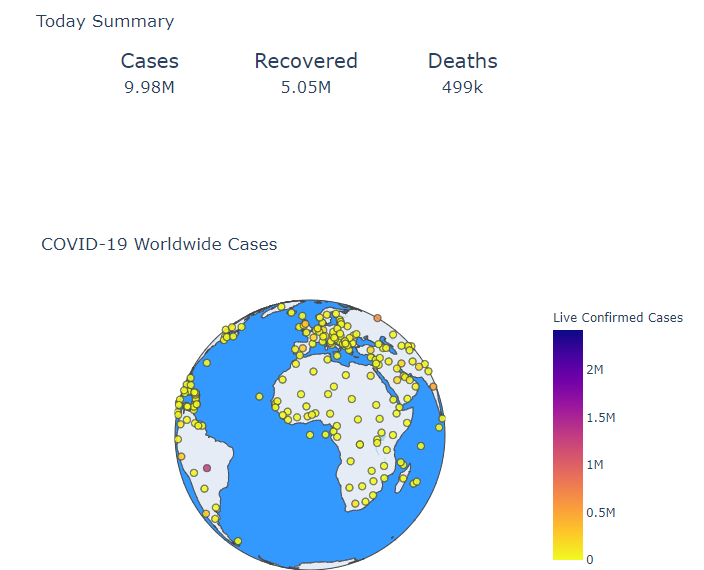
\includegraphics[width=11cm]{latex/images/world.PNG}%
    \caption{World Statistics Example}
    \label{world}
\end{figure}

These included:

\begin{itemize}
    \setlength\itemsep{-0.3cm}
    \item Record of the number of cases/recovered/deaths in the world up to date.
    \item Interactive world view of how the number of cases are spread around the word.
    \item Charts displaying what are today's top 10 countries for number of cases and deaths and how their numbers changed in the last 24 hours.
    \item Interactive animations displaying how Coronavirus spread across different countries over time.
\end{itemize}

The data used in order to create these charts, was provided by the Center for Systems Science and Engineering (CSSE) at Johns Hopkins University \cite{world_data} and automatically updated every 24hrs.

\subsection{Live World News and Sentiment Analysis}

This section was possible thanks to the use of the Python News API \cite{news}, making use of this API are in fact fetched every 2 hours news from a large number of countries around the world about Coronavirus. 

\begin{figure}[ht!]%
    \centering
    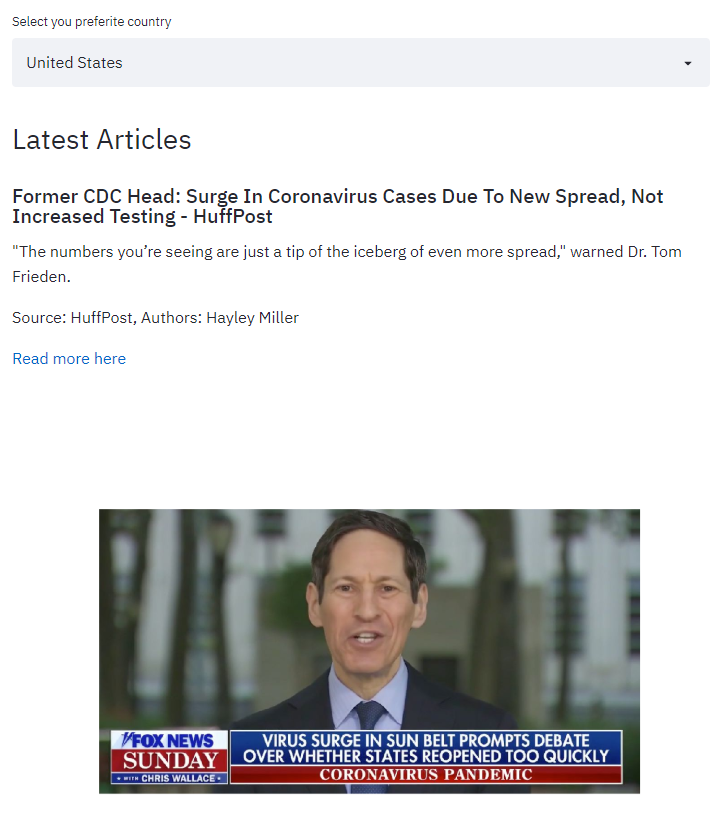
\includegraphics[width=9cm]{latex/images/news.PNG}%
    \caption{World News Example}
    \label{news}
\end{figure}

Using the fetched news article, it was then possible to apply sentiment analysis in each of the different countries in order to understand what are the key words of the day and what's the overall sentiment about the outbreak. Standard Natural Language Pre-processing techniques (eg. Tokenizzation, Stop Words Removal, Stemming) have been applied using the Python NLTK (Natural Language Toolkit) library and the sentiment was calculated using the VADER (Valence Aware Dictionary and sEntiment Reasoner) model. This type of model would then return a sentiment score between -1 (negative) and 1 (positive).

\begin{figure}[ht!]%
    \centering
    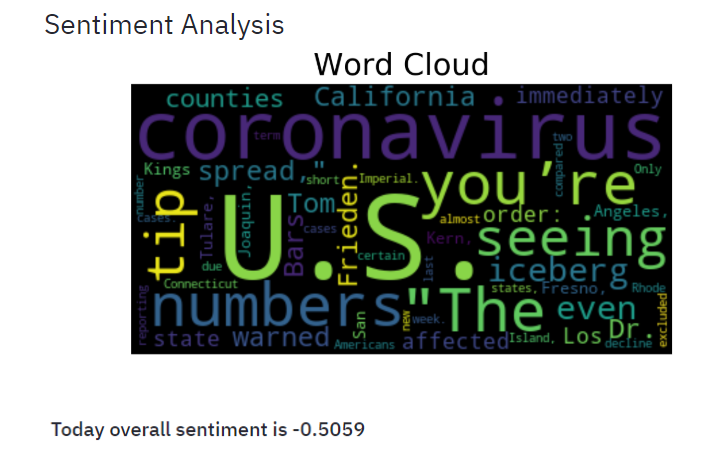
\includegraphics[width=10cm]{latex/images/news2.PNG}%
    \caption{World News Sentiment Analysis}
    \label{news2}
\end{figure}
